\section{Results} \label{sec:hResults}

All programs executed at least \num{4000} timesteps; they were compiled with CUDA v8 and \texttt{gcc v4.8.5}.
All programs were launched with \texttt{mpirun v3.1.4}.
Host-side memory management, grid generation, and initial conditions are not included in the timing measurement, but the measurement includes device-side global memory allocation and initial and final memory transfer between the host and device.
The heterogeneous swept rule algorithms and test cases were implemented in \texttt{hSweep v2.0}~\cite{hSweepz}.

\hfigs{BestRuntimeHeat}
{BestSpeedupHeat}
{Time cost of heat equation program at best launch condition.}
{Speedup of swept version at best launch condition.}
{Performance comparison of the hSweep heat equation programs.}

\hfigs{BestRuntimeEuler}
{BestSpeedupEuler}
{Time cost of Euler equation program at best launch condition.}
{Speedup of swept version at best launch condition.}
{Performance comparison of the hSweep Euler equations programs.}

We obtained the results presented here by running the \texttt{Classic} and \texttt{Swept}
programs on two nodes of the Oregon State University College of Engineering cluster.
Each node contains two sockets with~\CCPU{} processors containing ten cores each operating at~\SI{2.60}{\giga\hertz}.
An~\CGPU{} GPGPU is available to one of these nodes through a PCI connection.

Figure~\ref{f:BestRuntimeHeat} compares the computational time cost per time step
of the \texttt{Classic} and \texttt{Swept} algorithms applied to the heat equation.
These results are generally consistent with our expectations for several reasons.
First, we observe that in all previous experiments~\cite{OurJCP, alhubail:16jcp},
\texttt{Swept} achieves a period of strong speedup but reaches its asymptotic performance
at smaller grid sizes than \texttt{Classic}.
For \texttt{Classic} this occurs relatively soon after \texttt{Swept}, and the time cost of both algorithms with respect to grid size grows similarly so the relative speedup of \texttt{Swept} declines as well although the absolute speedup remains constant.

Second, although the minimum grid size in this study is about \tx{100} times larger
than our previous study, and the maximum grid size is about \tx{10} times larger,
Figure~\ref{f:BestSpeedupHeat} shows a remarkably similar trend in the speedup of swept decomposition.
In general the speedup exhibited by the heterogeneous case is \tx{2} the speedup at the analogous grid size in the GPU-only case over the experimental range.
The relative speedup of the swept rule is expected since the latency that our program avoids is a much larger cost in internode communication.

Figure~\ref{f:BestRuntimeEulerResult} compares the time cost per timestep of the \texttt{Classic} and \texttt{Swept} algorithms with the Euler equations and shows the same performance trends as the heat equation.
In this case, the communication costs that the program avoids are significant enough that swept decomposition provides a tangible benefit despite the extra complexity, management, and memory resources that it requires.
This shows that swept time-space domain decomposition is a viable method for complex equations in one dimension on systems with substantial communication costs and various architectures.

Figures~\ref{f:EulerContours} and~\ref{f:HeatContours} show contour maps of the results
of the complete experiment, as described at the end of Section~\ref{sec:ExpMethod}, on the equations.
By creating similar maps in the first stage of the experiment, we were able to narrow the range of possible best affinity values for all experimental settings and run an experiment with greater granularity in the affinity dimension.
In the interest of most accurately describing the performance of our program, we present the results of the final rather than the screening experiment.

Figure~\ref{f:EulerContours} shows interesting characteristics of the programs that vary by runtime configuration and decomposition method.
Notably, these results show that for the Euler equations, the \texttt{Swept} program often achieves best performance at GPU affinities between \numrange{45}{55} and often does best with \num{768} grid points in the domain of dependence, but performs particularly poorly with \num{512} points.
From other perspectives the performance profile of the \texttt{Swept} Euler equations program appears quite regular, so a sudden drop in performance followed by a substantial increase is unexpected.
The consistency of the influence of GPU affinity allows further studies to explore more granular performance characteristics.
While the saddle along the threads per block axis is problematic for our
general recommendations, we also observe that the program consistently exhibits similar performance from~\numrange{192}{384} threads per block.

Additionally, we observe from these maps that \texttt{Swept} produces a more orderly performance profile than \texttt{Classic}.
For grid sizes under \num{e6} spatial points, the classic decomposition technique produce peaks and valleys over a wide range of threads per block and GPU affinities.
On larger grids, that chaos regularizes and the best performance occurs with smaller grids and larger GPU affinities.
This suggests that we may have truncated the GPU affinity dimension prematurely in our experiments; however, from our observations we conclude that the best performance is well approximated by the experimental grid and that the most performative configuration overall will not lie far outside of the grid if it does.
The regularity we observe in the experimental grid for \texttt{Swept} programs also extends in the grid size dimension as described by Figures~\ref{f:BestRuntimeHeatResult} and \ref{f:BestRuntimeEulerResult} where swept decomposition produces a nearly perfect power law curve for each problem.
These figures show a significant improvement for \texttt{Swept} programs over \texttt{Classic} ones.
This relative advantage diminishes with greater problem sizes, but for the heat equation,  Figure~\ref{f:BestSpeedupHeat} shows an \tx{18} speedup at \num{5e5} spatial points falling to about a \tx{4} speedup at \num{e7}.

\begin{figure}[htbp]
    \centering
    \begin{subfigure}[t]{.75\textwidth}
        \centering
        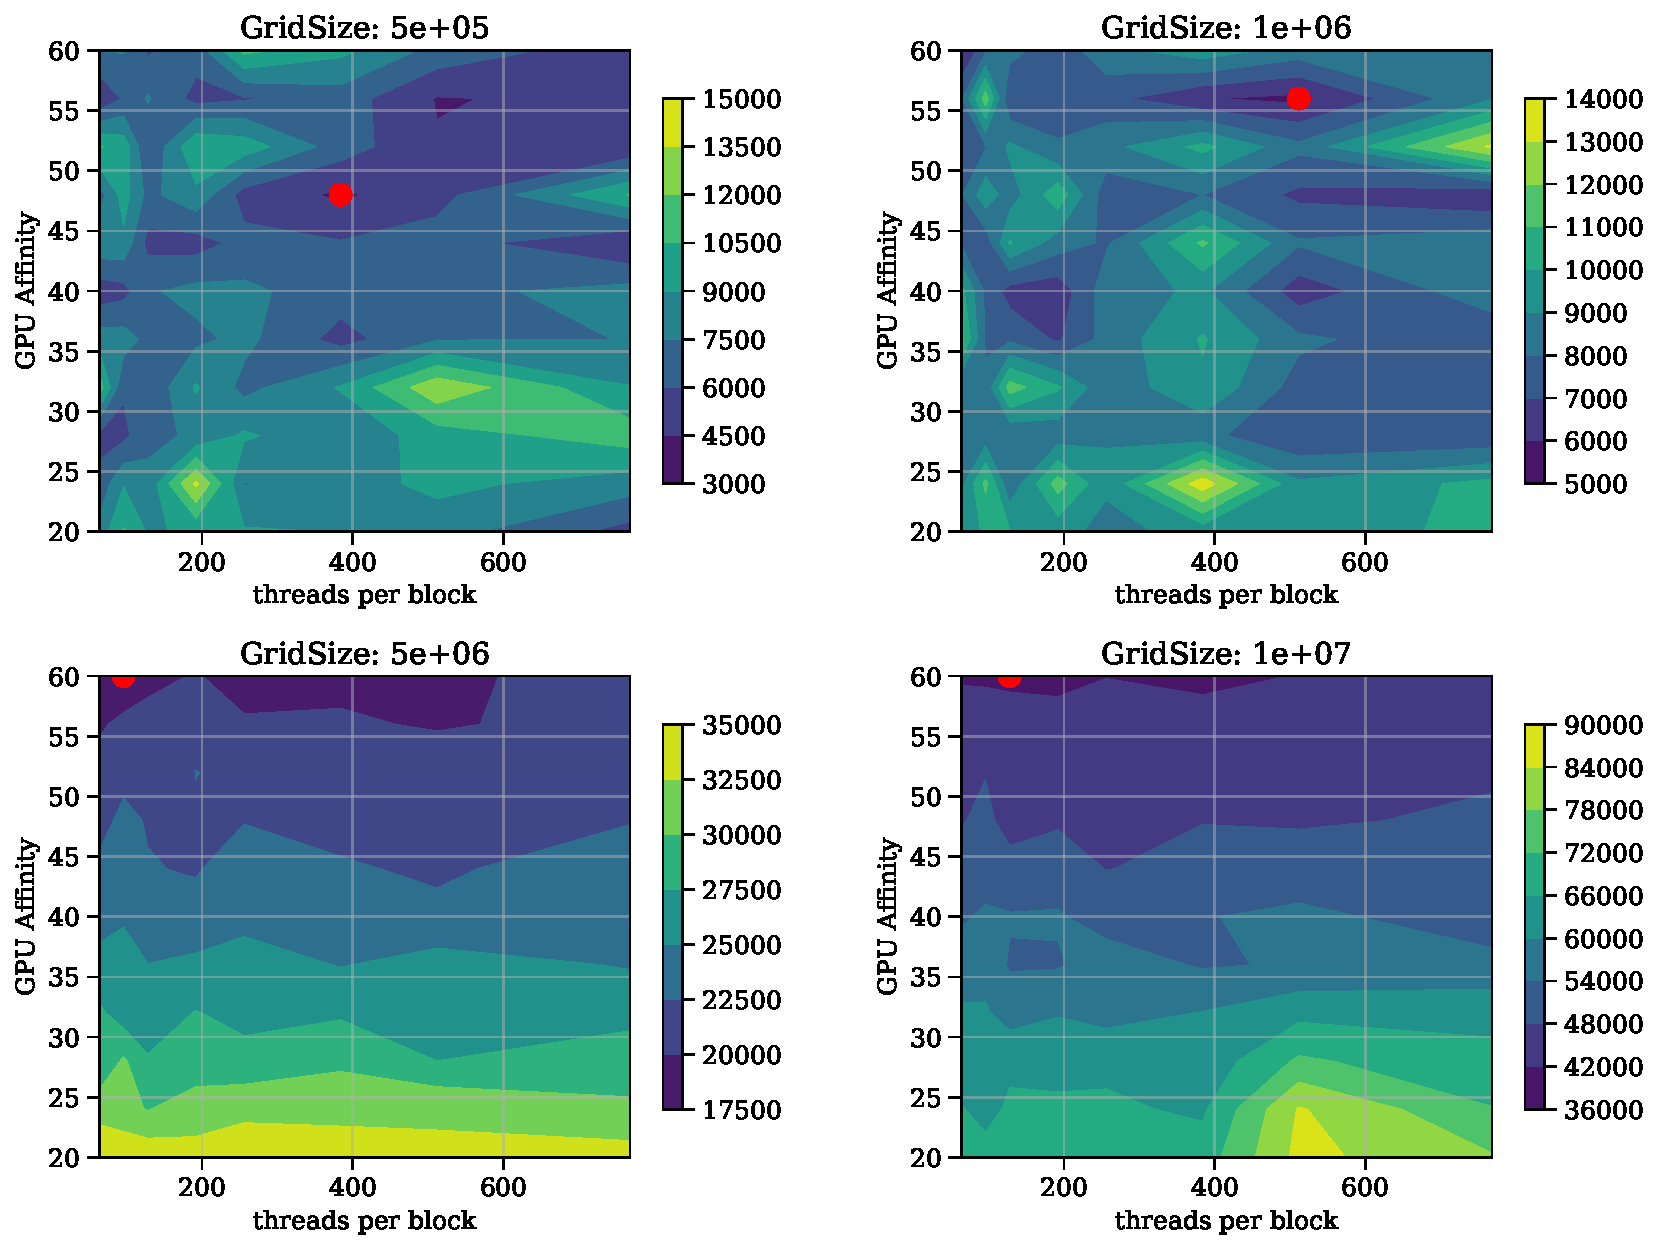
\includegraphics[width=\textwidth]{RawContourEulerClassictime}
        \caption{Classic decomposition}
        \label{f:EulerContourC}
    \end{subfigure}
    \begin{subfigure}[!tb]{.75\textwidth}
        \centering
        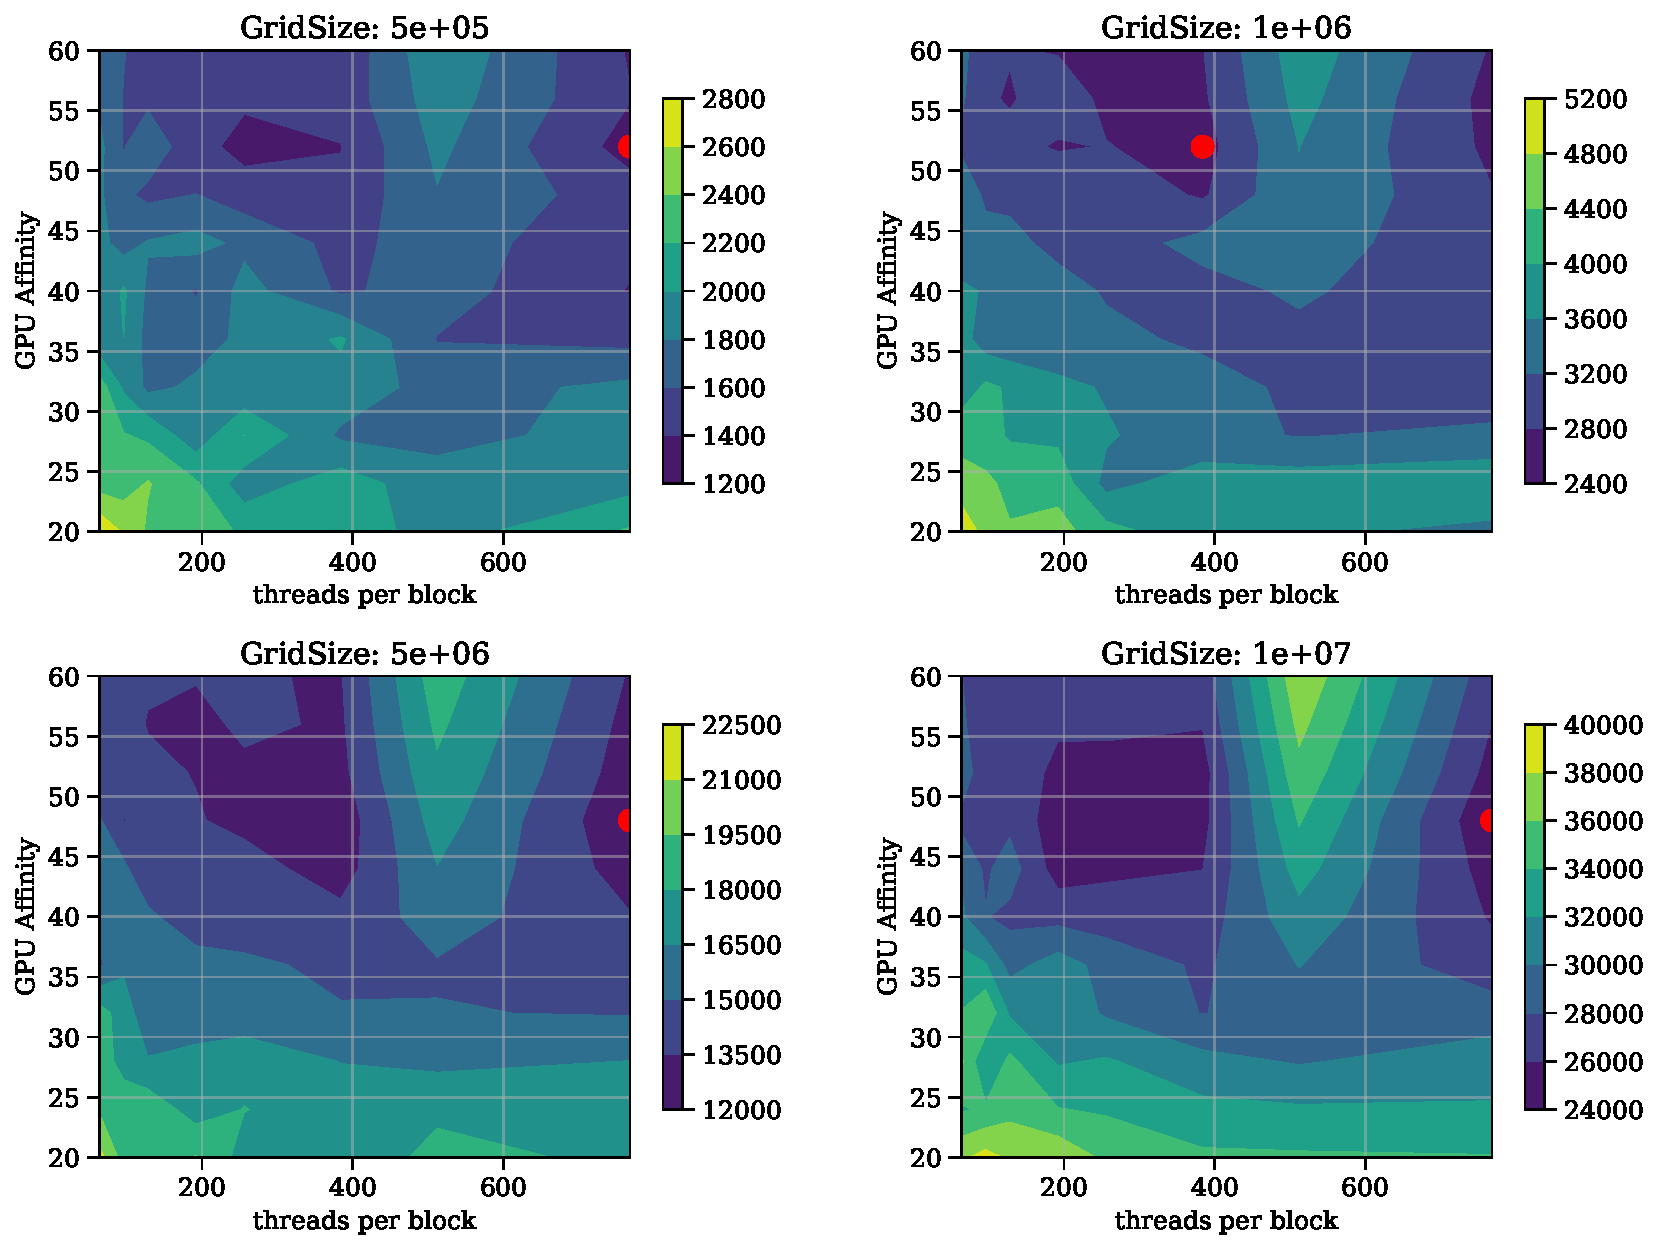
\includegraphics[width=\textwidth]{RawContourEulerSwepttime}
        \caption{Swept decomposition}
        \label{f:EulerContourS}
    \end{subfigure}
    \caption{A map of the time cost per timestep of the Euler equations at 4 grid sizes.
    The red dot signifies the best performance.}
    \label{f:EulerContours}
\end{figure}

\begin{figure}[htbp]
    \centering
    \begin{subfigure}[t]{.75\textwidth}
        \centering
        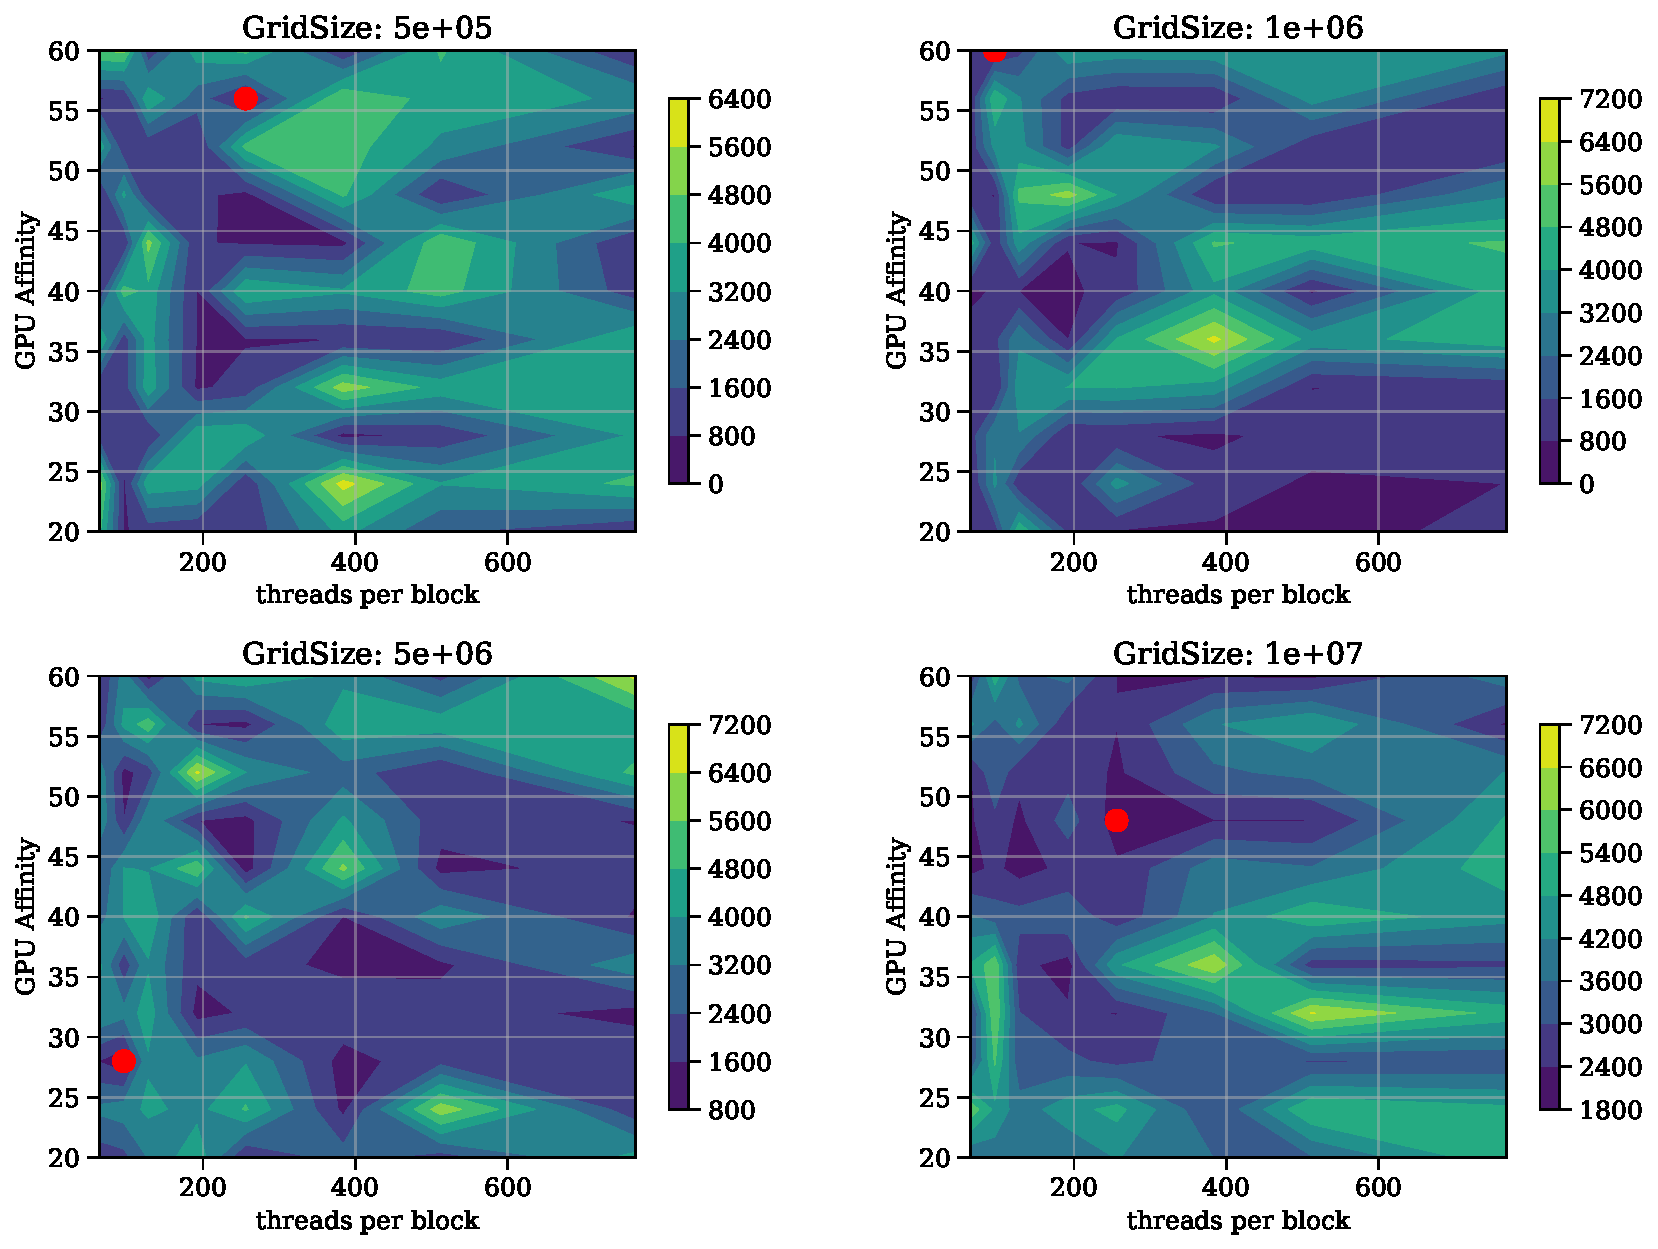
\includegraphics[width=\textwidth]{RawContourHeatClassictime}
        \caption{Classic decomposition}
        \label{f:HeatContourC}
    \end{subfigure}
    \begin{subfigure}[!tb]{.75\textwidth}
        \centering
        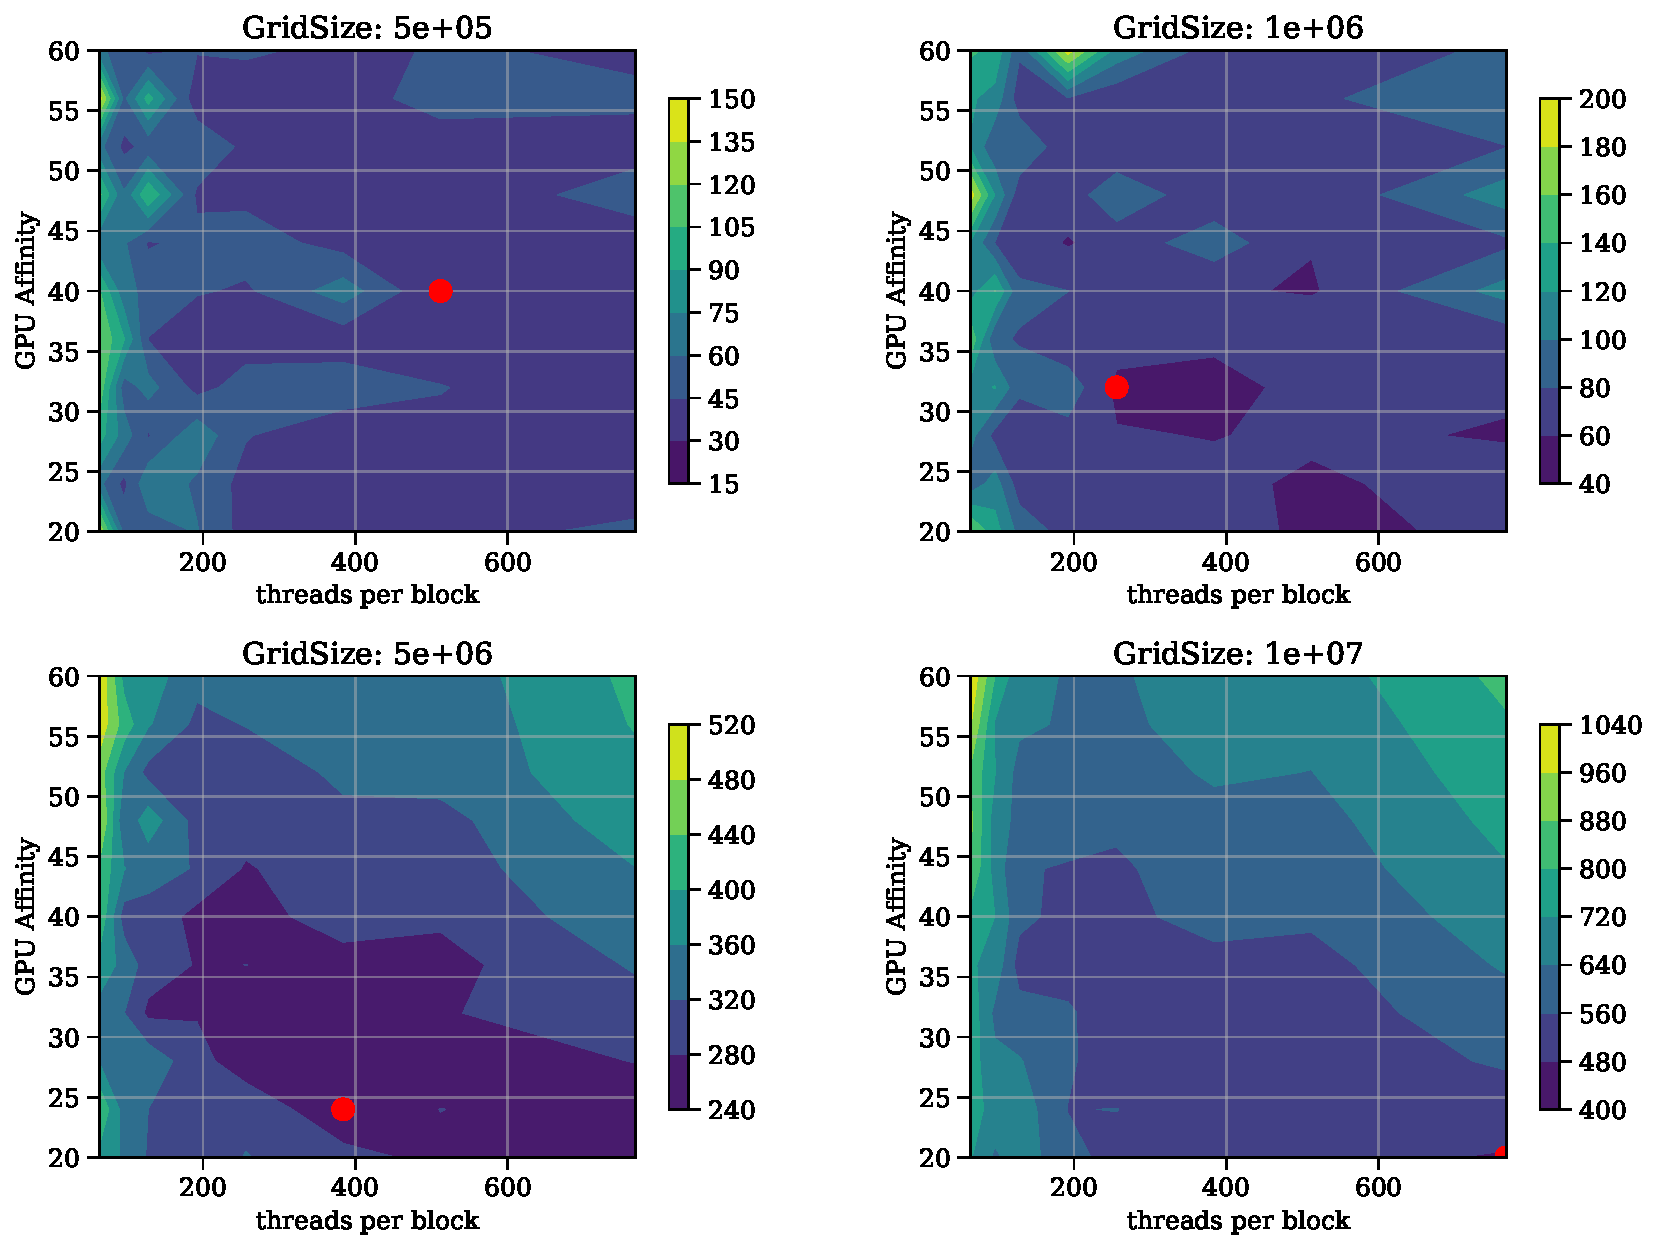
\includegraphics[width=\textwidth]{RawContourHeatSwepttime}
        \caption{Swept decomposition}
        \label{f:HeatContourS}
    \end{subfigure}
    \caption{A map of the time cost per time step of the heat equation at 4 grid sizes.
    The red dot signifies the best performance.}
    \label{f:HeatContours}
\end{figure}

Though we would emphasize that these results are representative of narrow experimental conditions,
architectures and design settings, the regularity of the \texttt{Swept} program performance
allows us to present fitted results in Table~\ref{tab:tablefit}, corresponding to the data points presented in Figures~\ref{f:BestRuntimeHeat} and ~\ref{f:BestRuntimeEuler}, that may illuminate and
guide future work on this and similar topics.

\begin{table}
\caption{Coefficients for power-law fit of grid size vs time per timestep ($y = Ax^b$) of \texttt{Swept} performance at best runtime configuration.}
%\vspace{-0.5em}
\label{tab:tablefit}
        \begin{center}
                \begin{tabular}{@{}l c c c}
                \toprule
                Equation & A & b & $R^2$ \\
                \midrule
                Euler   & \num{3.55e-3} & \num{0.976} & \num{0.999} \\
                Heat    & \num{1.08e-4} & \num{0.949} & \num{0.999} \\
                \bottomrule
                \end{tabular}
        \end{center}
\end{table}
